\documentclass[12pt]{article}
\usepackage{amsmath,amsfonts,amssymb}
\usepackage{graphicx}
\usepackage{hyperref}
\usepackage{authblk}

\title{Observer-Centric Bitstring Universes: A Minimal Informational Model of Reality}
\author{Juha Meskanen}
\date{July 2025}

\begin{document}

\maketitle

\begin{abstract}
    We present a discrete, observer-based model of the universe grounded in bitstring information theory. In this minimal setting, we define observers as sequences of finite bitstrings and investigate their persistence within possible universes composed of frames of bits. The model introduces a similarity metric for observer survival, proposes an entanglement-like phenomenon via shared memory fragments, and reinterprets the wavefunction as a compressed extrapolation over observer trajectories. This framework challenges traditional physical ontology, suggesting that reality is observer-centric and informational at its core.
\end{abstract}

\section{Introduction}

We explore a radically minimalist foundation for physics based on bitstrings and observer-centric reasoning. In this model, the universe is not something that evolves over time according to dynamical rules, but rather a collection of static information patterns in which observers find themselves embedded. Observers persist through time only by re-identifying themselves across similar structures. Thus, what we call \emph{reality} is the subset of bitstring universes that contain coherent observer trajectories.

\section{Framework and Definitions}

Let $B$ denote the total number of bits used to describe a universe. We define:

\begin{itemize}
    \item $\mathcal{U}_B$: the set of all possible universes composed of bitstrings of length $B$, partitioned into frames $f_i$ representing temporal slices.
    \item $O = \{o_1, o_2, \ldots, o_n\}$: a sequence of bitstrings representing the observer's memory and state across subjective time.
\end{itemize}

\subsection{Observer-Centric Universe Construction Principle (OCUCP)}

An observer is said to exist only in those universes $U \in \mathcal{U}_B$ such that for all $i$, there exists $o_i \subseteq f_i$. That is, the observer must be embedded, frame by frame, into the universe.

This approach inverts the usual ontology: rather than universes determining observers, observers determine which universes are relevant. Reality is defined \emph{relative to the observer's compatibility with the universe}.

\subsection{Observer Memory Lemma (OML)}

Let $O = \{o_1, o_2, \ldots, o_n\}$ be an observer trajectory, and $F = \{f_1, f_2, \ldots, f_n\}$ a candidate sequence of universe frames. Then, the observer can only \emph{remember} or \emph{experience} $F$ if:

\[
    \exists\ \epsilon > 0\ \text{ such that }\ \text{Similarity}(o_i, f_i) \ge \epsilon\ \text{ for all } i.
\]

In other words, the observer's internal structure must sufficiently overlap with the universe frames for continuity and memory to be possible. Memory is defined as structural self-similarity over time, not as causal flow.

\subsection{Similarity Metric and Observer Survival}

We define a similarity function $\text{Sim}(a, b)$ between two bitstrings. An observer $O$ survives a frame transition $o_i \to o_{i+1}$ only if $\text{Sim}(o_i, o_{i+1}) \ge \delta$ for some threshold $\delta$. This defines a selection criterion over possible trajectories.

\section{Compression and the Wavefunction}

We propose a new interpretation of the quantum wavefunction grounded in the logic of observer survival through compression.

\subsection{Compression Bias Principle (CBP)}

Let $C(F)$ denote the compressed length of a sequence of universe frames $F = \{f_1, \ldots, f_n\}$. Then, the number of observers that can embed within $F$ is inversely correlated with $C(F)$.

That is, smooth, regular, and compressible universes support more observers, simply because more observer trajectories can be accommodated within the same limited bit budget. Consequently, the universe we find ourselves in is likely to be highly compressible.

\subsection{Wavefunction as Compressed Continuation}

An observer predicts future frames by extrapolating structural regularities from memory using compression-based logic:

\begin{itemize}
    \item The observer contains past states $\{o_1, \ldots, o_t\}$.
    \item It extrapolates possible futures $o_{t+1}, \ldots, o_{t+k}$ using pattern completion.
    \item If the compression basis is Fourier/sine-based (e.g., JPEG), extrapolation leads to smooth predictions.
    \item Multiple continuations are possible, forming a "superposition" within the observer's internal model.
\end{itemize}

Interference arises when extrapolated continuations reuse shared substrings. Thus, quantum phenomena emerge not from physical superposition, but from ambiguous extrapolations under compression logic. This model views the wavefunction as an efficient coding scheme, not as a physical entity.

\section{Entanglement and Shared Memory}

Entanglement is modeled as mutual constraint between observer subcomponents. If two observer bitstrings $A$ and $B$ share internal fragments and exist within a common universe $U$, then the observer can only survive in frames that preserve both. This shared structure constrains joint probabilities, introducing entanglement.

This is a structural, non-local correlation—not a causal interaction. It arises because the observer is a unified bitstring with branching substructures, not two separate agents.

\section{Simulation}

We present a simulation framework that implements the observer-centric model of universes. The simulation generates two-dimensional discrete spacetimes as sequences of bitstrings, allowing observers to navigate these universes based on their memory patterns.

The simulation software implements the observer-centric model as follows:

\begin{itemize}
    \item \textbf{Bitstring Universe:} Generate all possible spacetime configurations as sequences of $n$-bit states over time.
    \item \textbf{Observers as Substrings:} Define an observer as a recurring bit pattern and use substring matching to detect compatible histories.
    \item \textbf{Similarity Score:} Score each universe path by how often the observer pattern appears, or by a more refined memory-similarity metric.
\end{itemize}

The program is hosted at:
\[
    \texttt{http://github.com/juham/simulations/paper4/observer\_centric\_universe.py}
\]

It takes the following input parameters:

\begin{itemize}
    \item Bit length $B$ of the universe.
    \item Number of frames $N$ to simulate, representing temporal evolution.
    \item List of observer bitstrings $O$, describing the evolution of observer memory and simpler particle bitstrings.
    \item Similarity threshold $\delta$ for observer survival.
\end{itemize}

The simulation generates a universe by randomly constructing frames of bits and then checks for observer compatibility. It tracks the evolution of observers across frames, visualizing their persistence and trajectories.

\begin{figure}[h!]
    \centering
    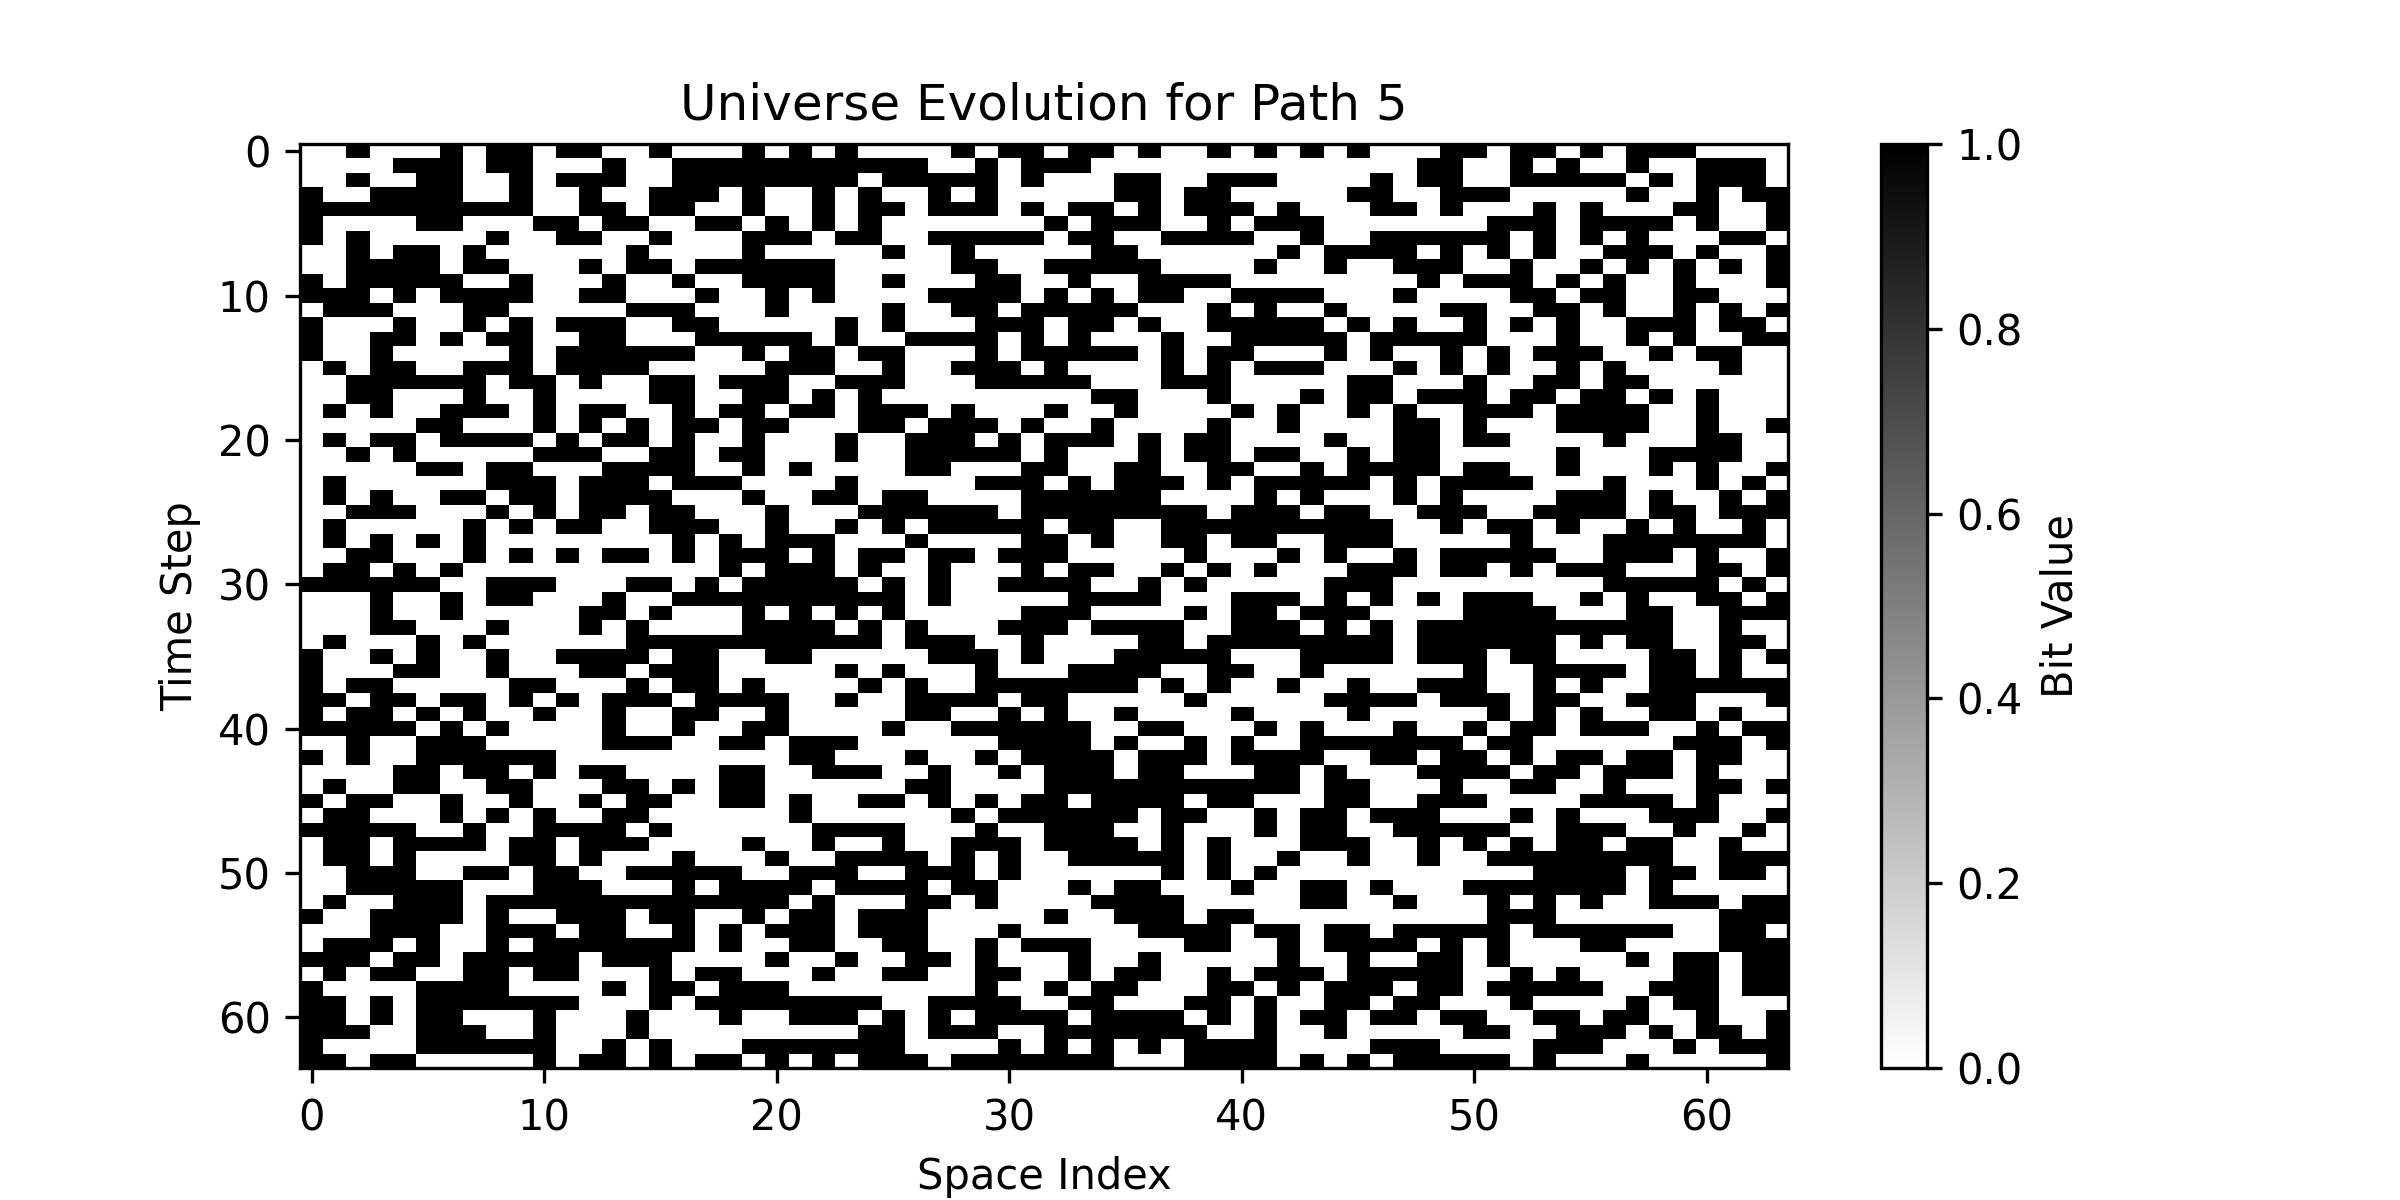
\includegraphics[width=1.0\textwidth]{figures/state_evolution_heatmap.png}
    \caption{State evolution of one of the simulated universes, including an observer. The evolution demonstrates coherence.}
    \label{fig:state_evolution}
\end{figure}

Particle trajectories are visualized as traces through the universe frames, showing how observers navigate the bitstring landscape. The simulation demonstrates that smooth trajectories can emerge when observers follow consistent patterns, even in a discrete universe.

\begin{figure}[h!]
    \centering
    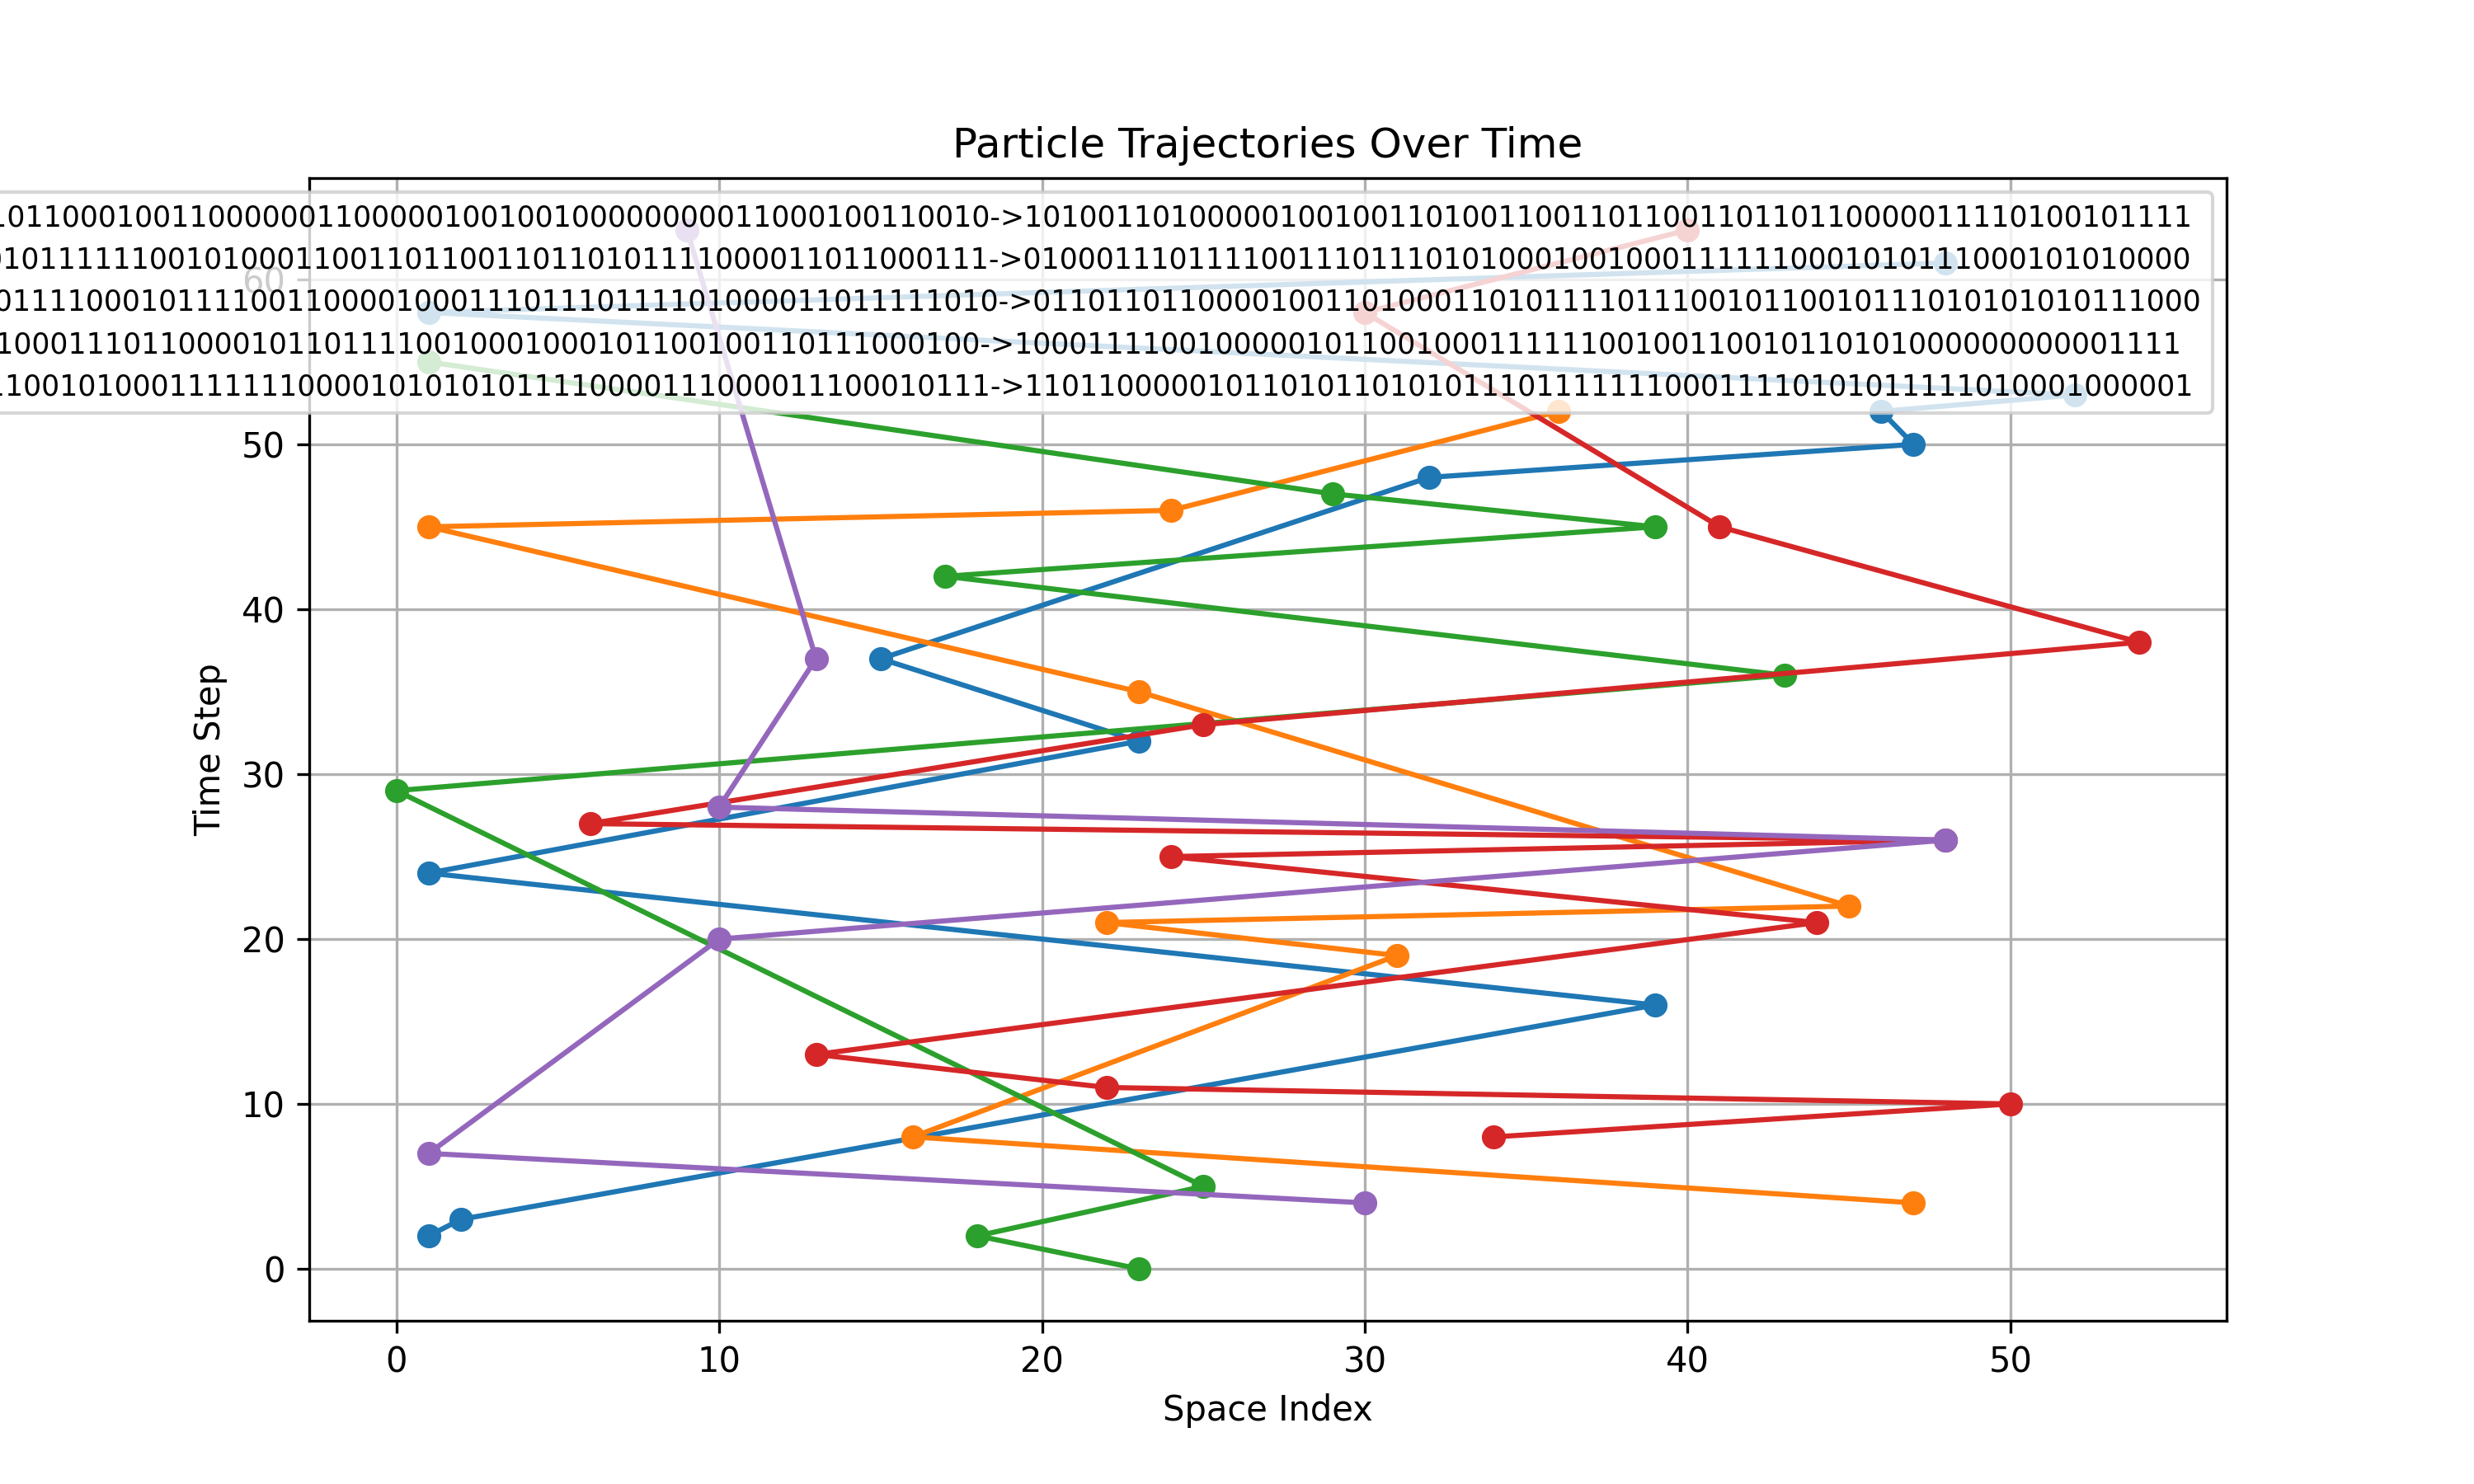
\includegraphics[width=1.0\textwidth]{figures/particle_trajectories.png}
    \caption{Particle traces showing that smooth trajectories emerge in universes that include coherent observer patterns.}
    \label{fig:particle_trajectories}
\end{figure}

A heatmap is generated to visualize the dynamics of the universe. Regions of high intensity indicate greater dynamical activity.

\begin{figure}[h!]
    \centering
    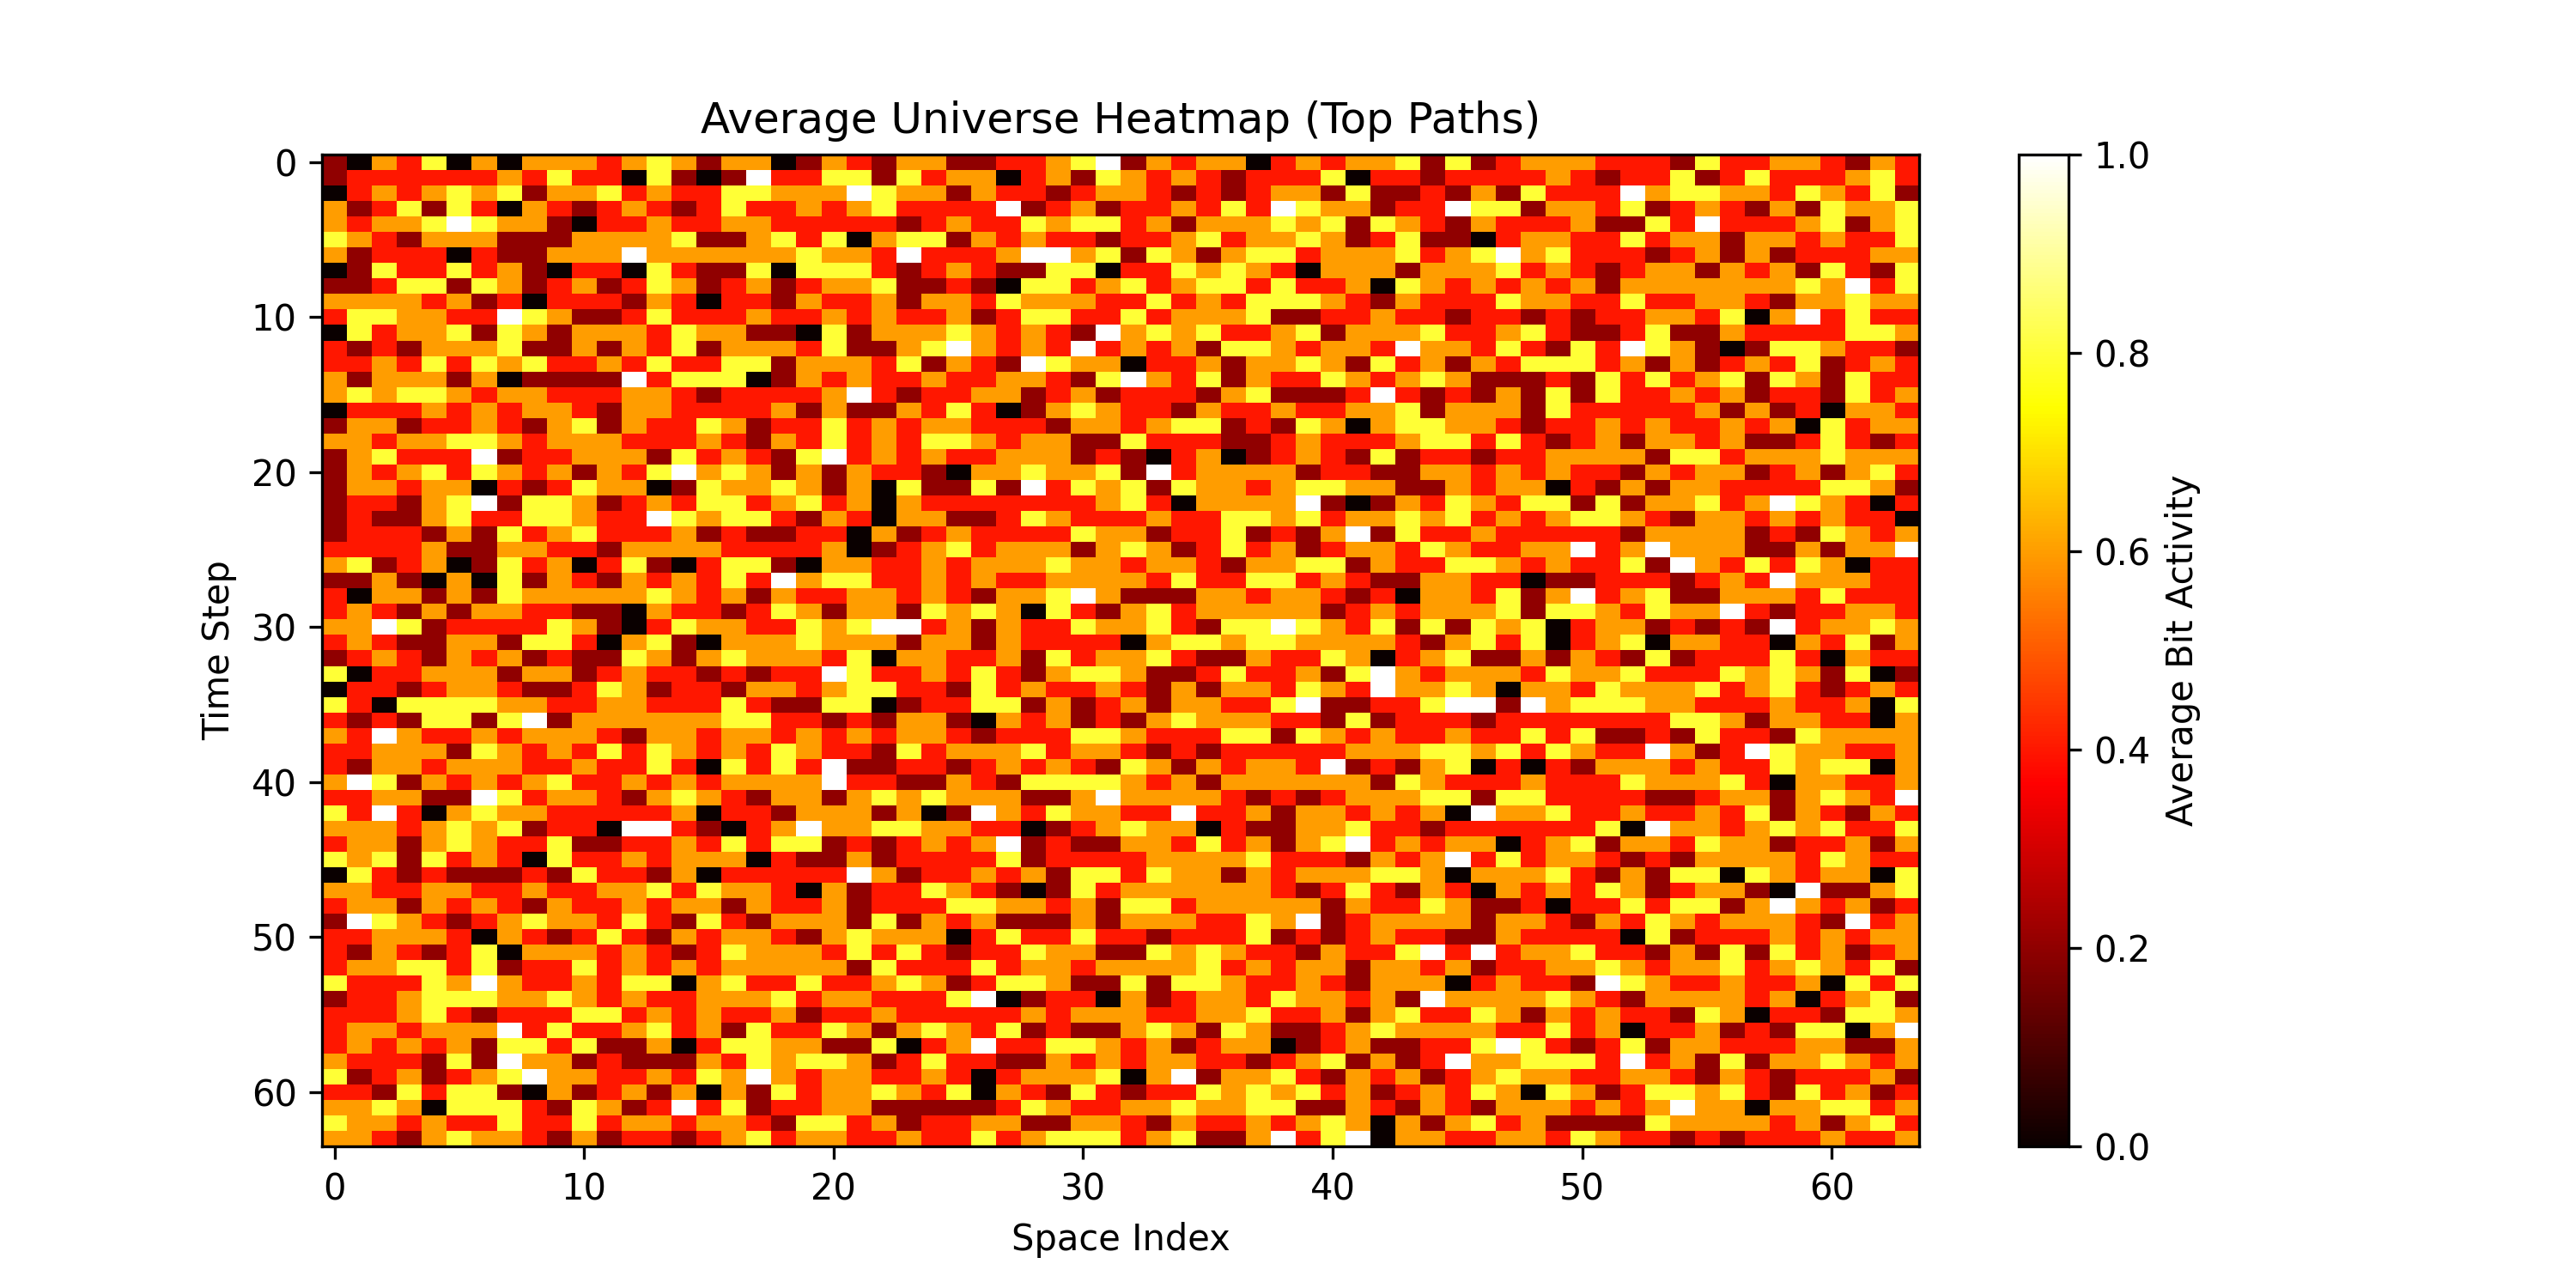
\includegraphics[width=1.0\textwidth]{figures/average_universe_heatmap.png}
    \caption{Heatmap visualizing the dynamics of the universe. Areas with a low density of particle trajectories indicate stable regions that change little over time. These worldlines are where observers or particles find consistent continuations.}
    \label{fig:average_universe_heatmap}
\end{figure}

\subsection{Wavefunction and Interference}

Why do we observe wave-like behavior in quantum mechanics? The wavefunction arises from the need to compress data. As the simplest periodic function, the sine wave offers an efficient basis for extrapolation. Observers prefer universe paths that align well with such wavefunctions, since those paths require fewer bits to describe. Universes with such structure are more probable because they support a greater number of embedded observers.

Interference emerges naturally when multiple such sine waves are superposed. Some paths reinforce alignment; others cancel. This mimics the Born rule of quantum mechanics: high amplitude corresponds to high probability, while destructive interference results in observer-incompatible paths.

\begin{figure}[h!]
    \centering
    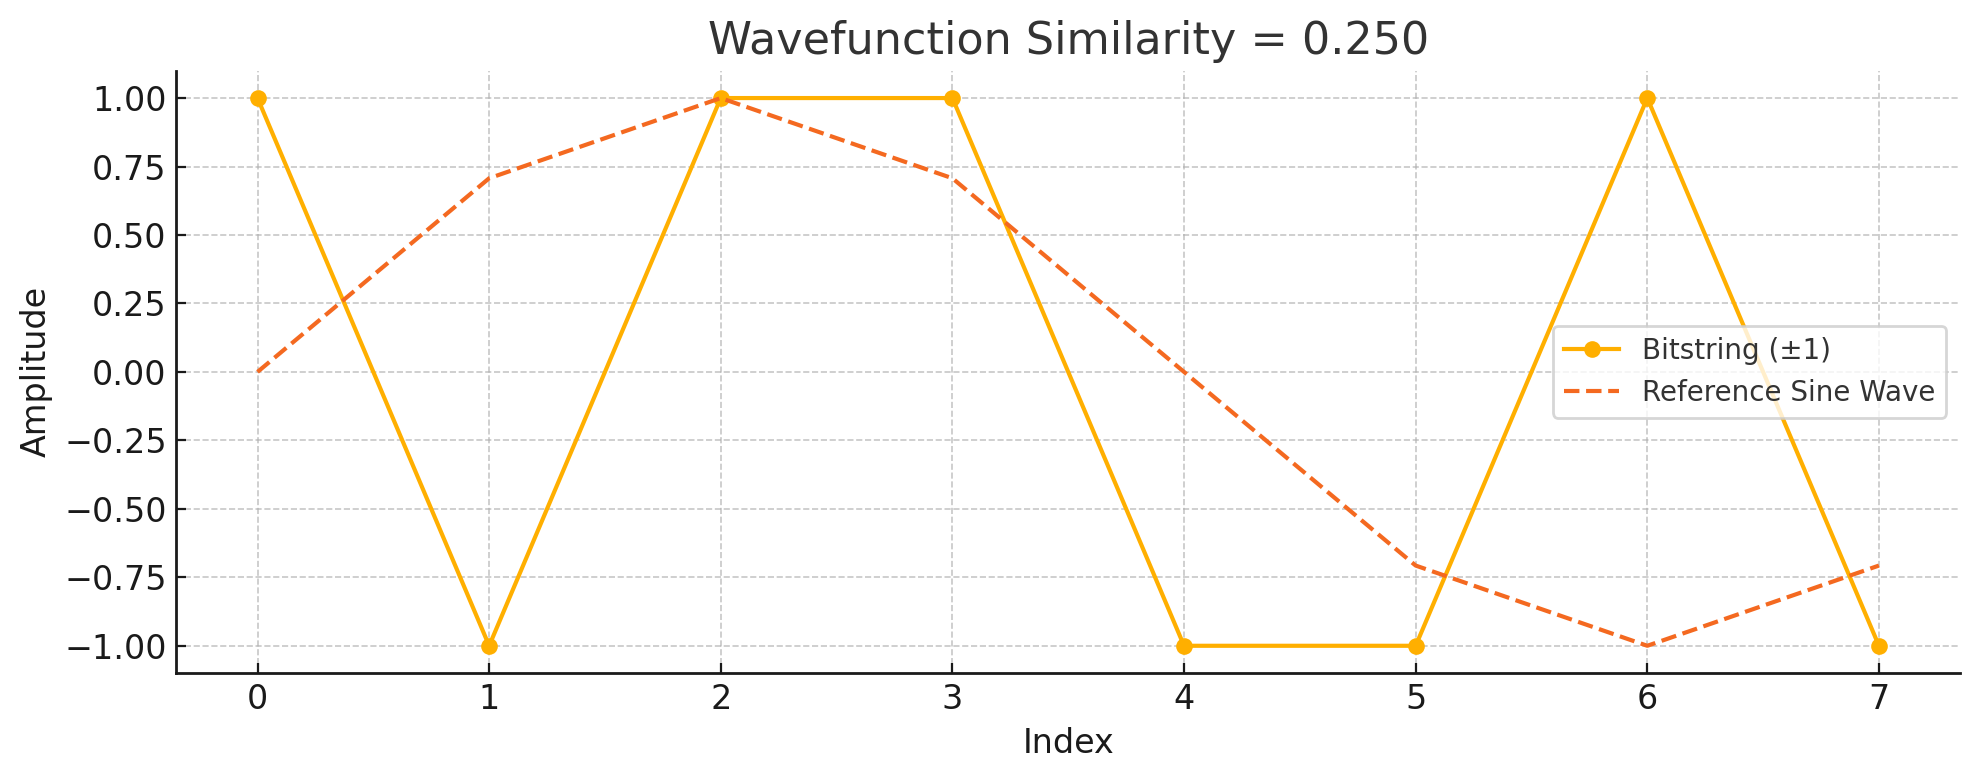
\includegraphics[width=1.0\textwidth]{figures/wavefunction_similarity.png}
    \caption{The chart shows how a bitstring (converted to ±1 amplitudes) aligns with a reference sine wave.
        The wavefunction similarity is calculated as the normalized dot product between these two curves.}
    \label{fig:wavefunction_similarity}
\end{figure}


This framework lets us interpret similarity as interference amplitude: when it's high, the observer's pattern resonates with a compressible (wave-like) universe. This links bit-level structure to emergent wavefunction behavior.

\begin{figure}[h!]
    \centering
    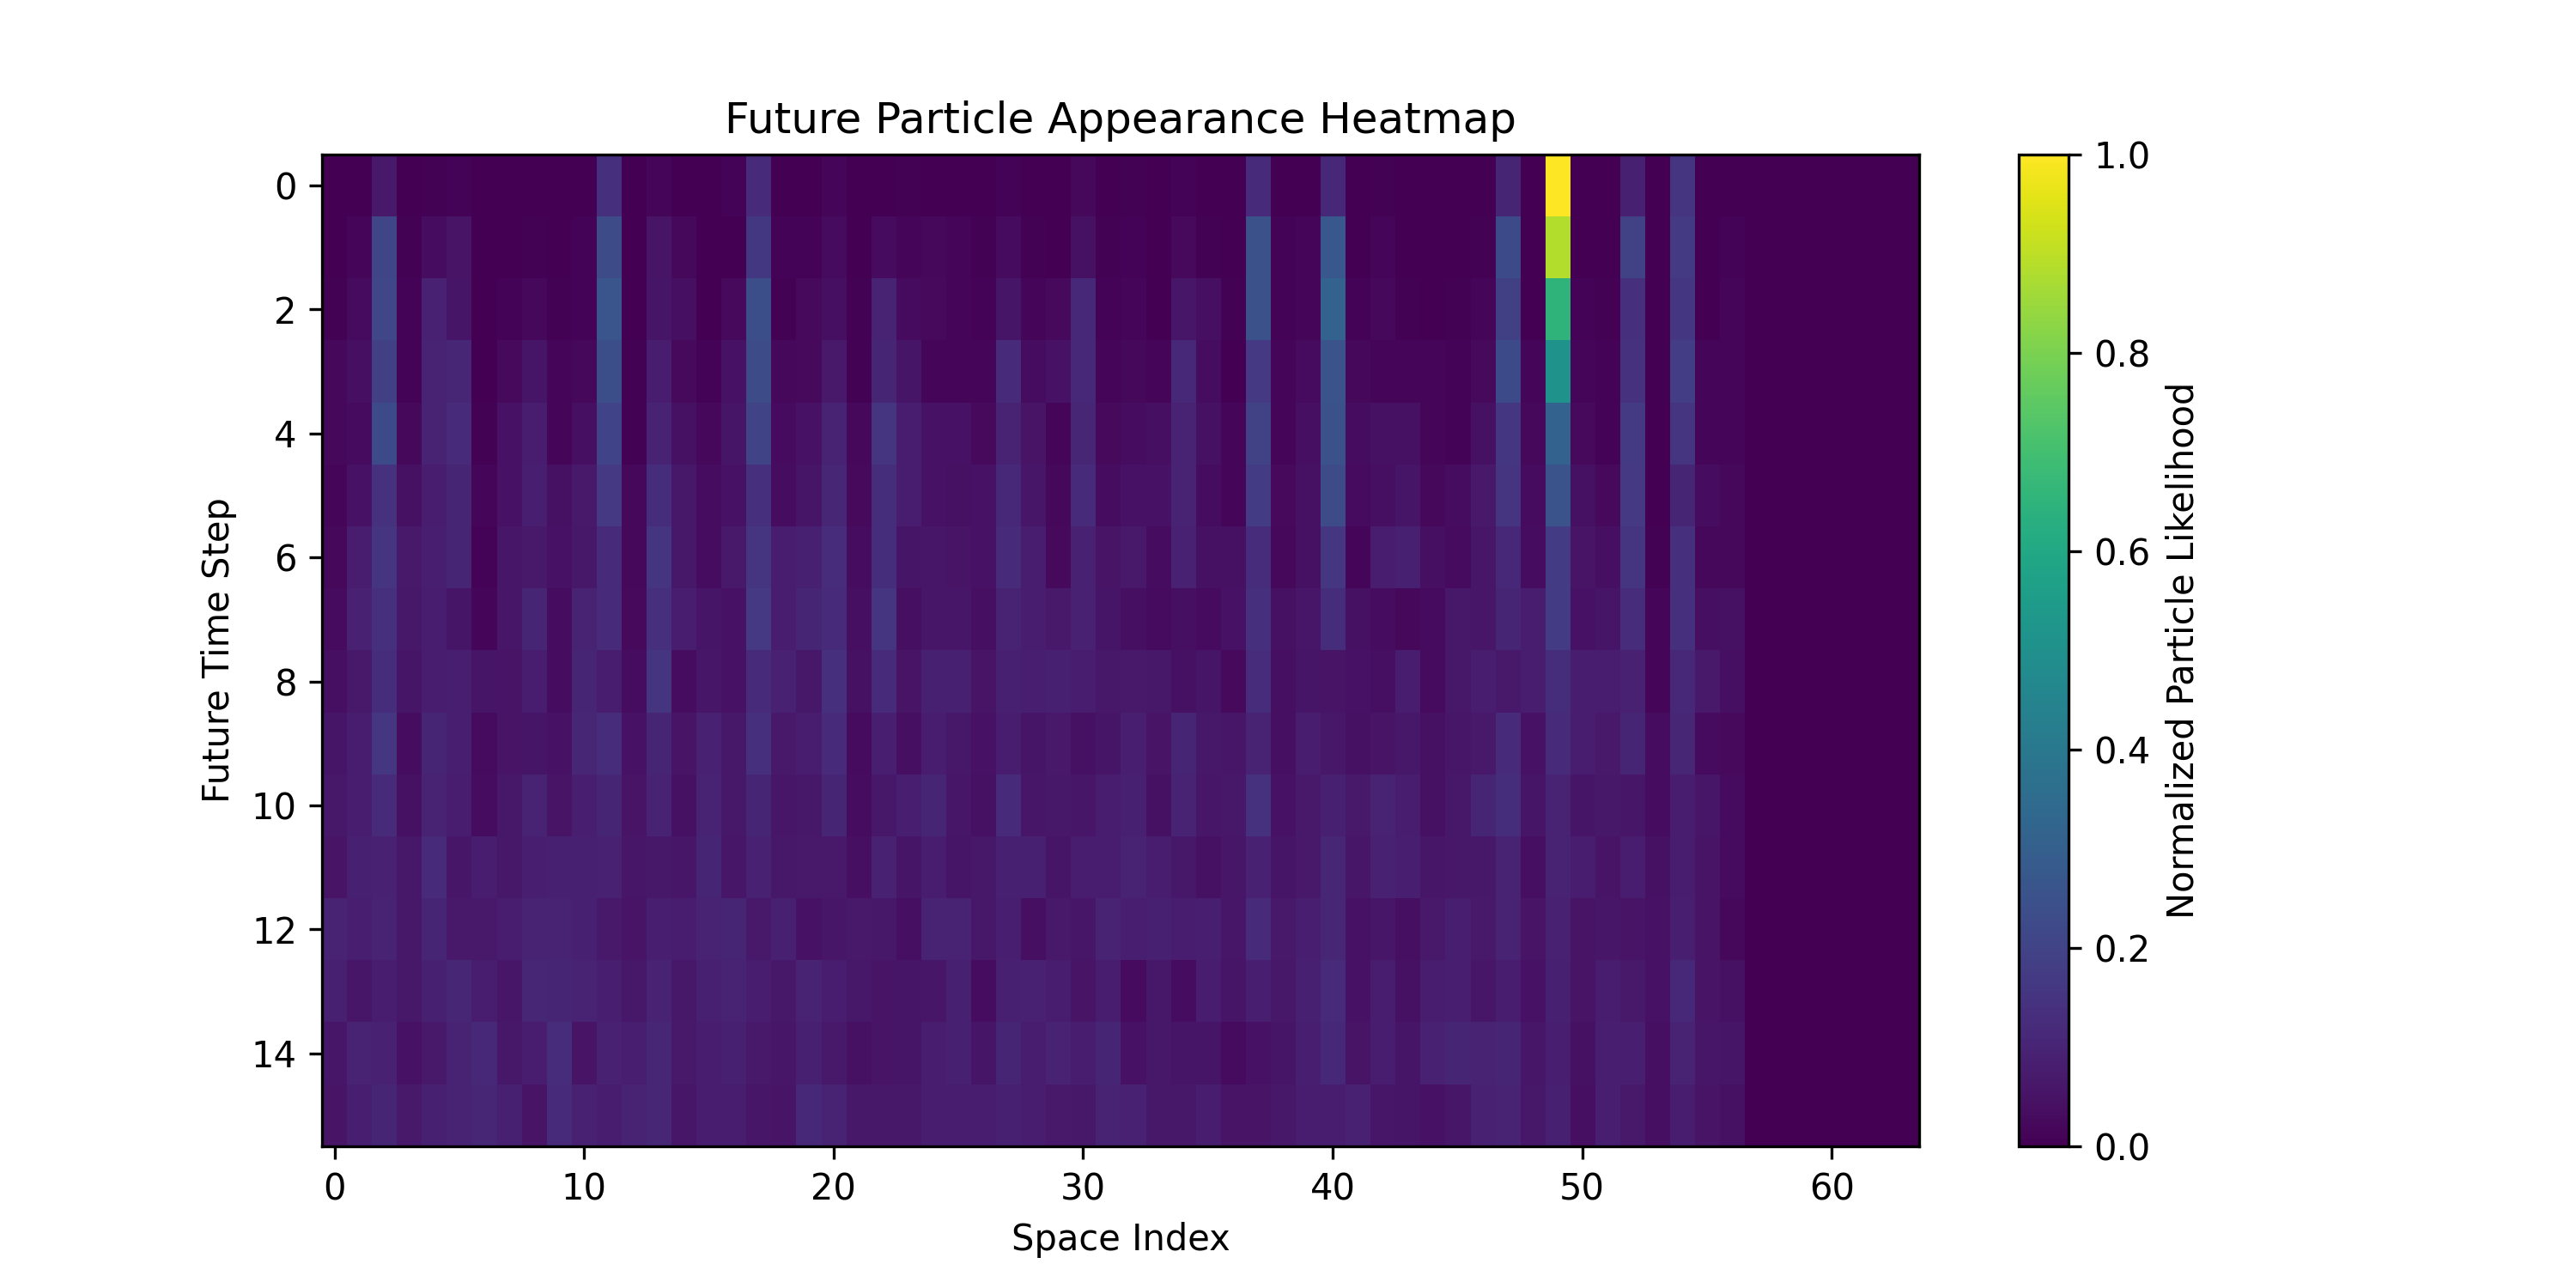
\includegraphics[width=1.0\textwidth]{figures/future_particle_heatmap.png}
    \caption{Heatmap visualizing possible future worlds. The image shows the density of particle trajectories in the future, indicating where observers or particles are likely to find consistent continuations. The future is not a single path but a set of probable continuations shaped by the observer's past. Predictability fades with distance from the current state as possible continuations proliferate.}
    \label{fig:future_particle_heatmap}
\end{figure}

\section{Discussion and Implications}

This model abandons conventional notions of causality and dynamics in favor of a static informational ontology. Universes do not evolve; rather, they are favored by observers based on structural compatibility. The past is defined by memory fragments; the future is an extrapolation constrained by compression logic.

There is no fundamental substrate—only bitstrings and the observer's search for consistent continuations. Gravity, time, and quantum effects emerge as statistical preferences under this framework.

\section{Conclusion}

We have proposed a minimal observer-centric framework in which the universe is composed of bitstrings, and persistence is governed by similarity and compression. Observer memory is realized through structural overlap, and probability emerges from counting consistent embeddings. This framework offers a possible foundation for reconciling quantum and classical perspectives under informational realism.

\end{document}
